%--------------------------------------------------------------- %
\documentclass[SPC-MASTER.tex]{subfiles}
\begin{document}
\Large
\section{CUSUM Charts}
\begin{itemize}
\item CUSUM charts, while not as intuitive and simple to operate as Shewhart charts, have been shown to be more efficient in detecting small shifts in the mean of a process. \item In particular, analyzing ARL's for CUSUM control charts shows that they are better than Shewhart control charts when it is desired to detect shifts in the mean that are 2 sigma or less.
\end{itemize}



% http://www.itl.nist.gov/div898/handbook/pmc/section3/pmc323.htm

\begin{figure}[h!]
\centering
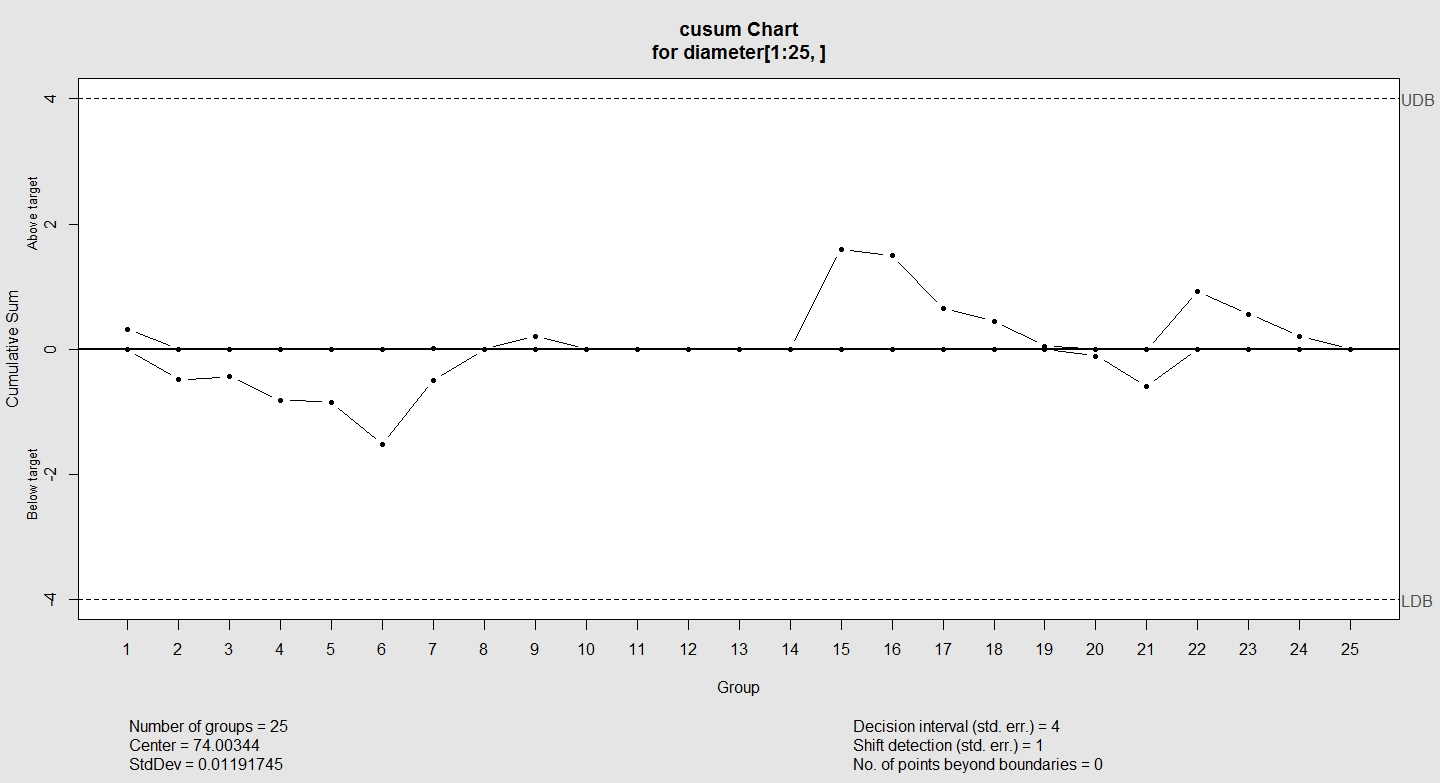
\includegraphics[width=0.7\linewidth]{images/CUSUMorings1}
\caption{}
\label{fig:CUSUMorings1}
\end{figure}

\begin{figure}[h!]
\centering
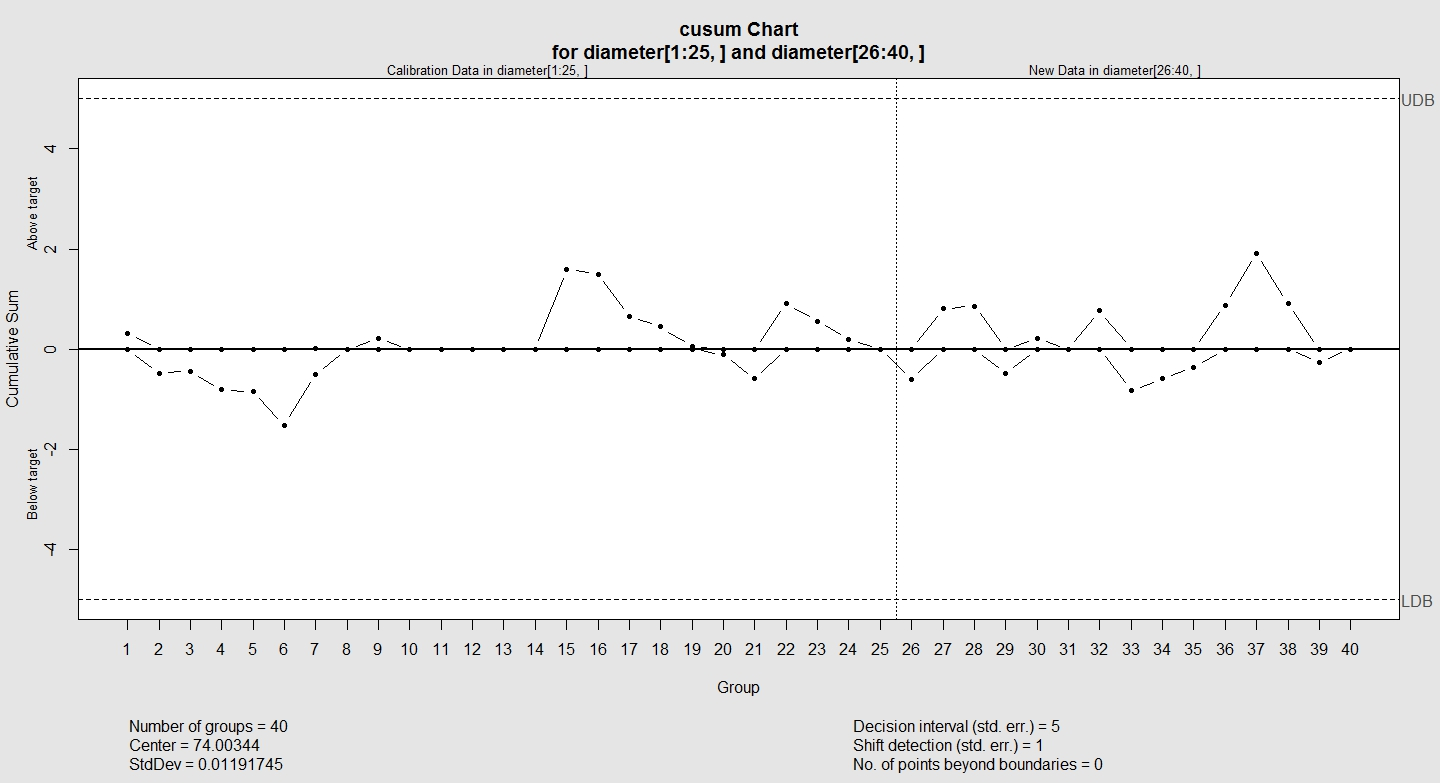
\includegraphics[width=0.7\linewidth]{images/CUSUMorings2}
\caption{}
\label{fig:CUSUMorings2}
\end{figure}

\section{The CUSUM chart}

Although the Shewhart chart is sensitive to sudden and large changes in measurement, it is ineffective in detecting small but persistent departure from the bench mark. For this, the CUSUM chart is more appropriate.

CUSUM is short for cumulative sums. As measurements are taken, the difference between each measurement and the bench mark value is calculated, and this is cumulatively summed up (thus CUSUM). If the processes are in control, measurements do not deviate significantly from the bench mark, so measurements greater than the bench mark and those less than the bench mark averaged each other out, and the CUSUM value should vary narrowly around the bench mark level. If the processes are out of control, measurements will more likely to be on one side of the bench mark, so the CUSUM value will progressively depart from that of the bench mark.

CUSUM is therefore conceptually simple. The statistical calculations involved are needed to make the method usable in practice, and they are as follows.

The first is to make the CUSUM line stable. As the number of measurements are taken, the probability that the CUSUM value may drift into extreme values increases. This is corrected by adjusting the CUSUM by an out of control criteria \textbf{k}, and resetting the CUSUM value whenever it crosses the bench mark value.

The consequence of this is that two sets of CUSUM values are available, 
\begin{itemize}
	\item one marks departures in excess of bench mark value, 
	\item and the other marks departures below the bench mark value.
\end{itemize}


The second is when to decide that the process is out of control and raise the alarm. This is set by a decision value above or below the bench mark \textbf{h}, and the out of control decision can be made when the CUSUM value reaches \textbf{h}.


This \textbf{h} really depends on how sensitive the user wishs the method to be. The more sensitive (the closer \textbf{h} is to the bench mark), the quicker will any departure from the bench mark be detected, but also the more likely a false alarm will occur.
\newpage
\begin{figure}[h!]
\centering
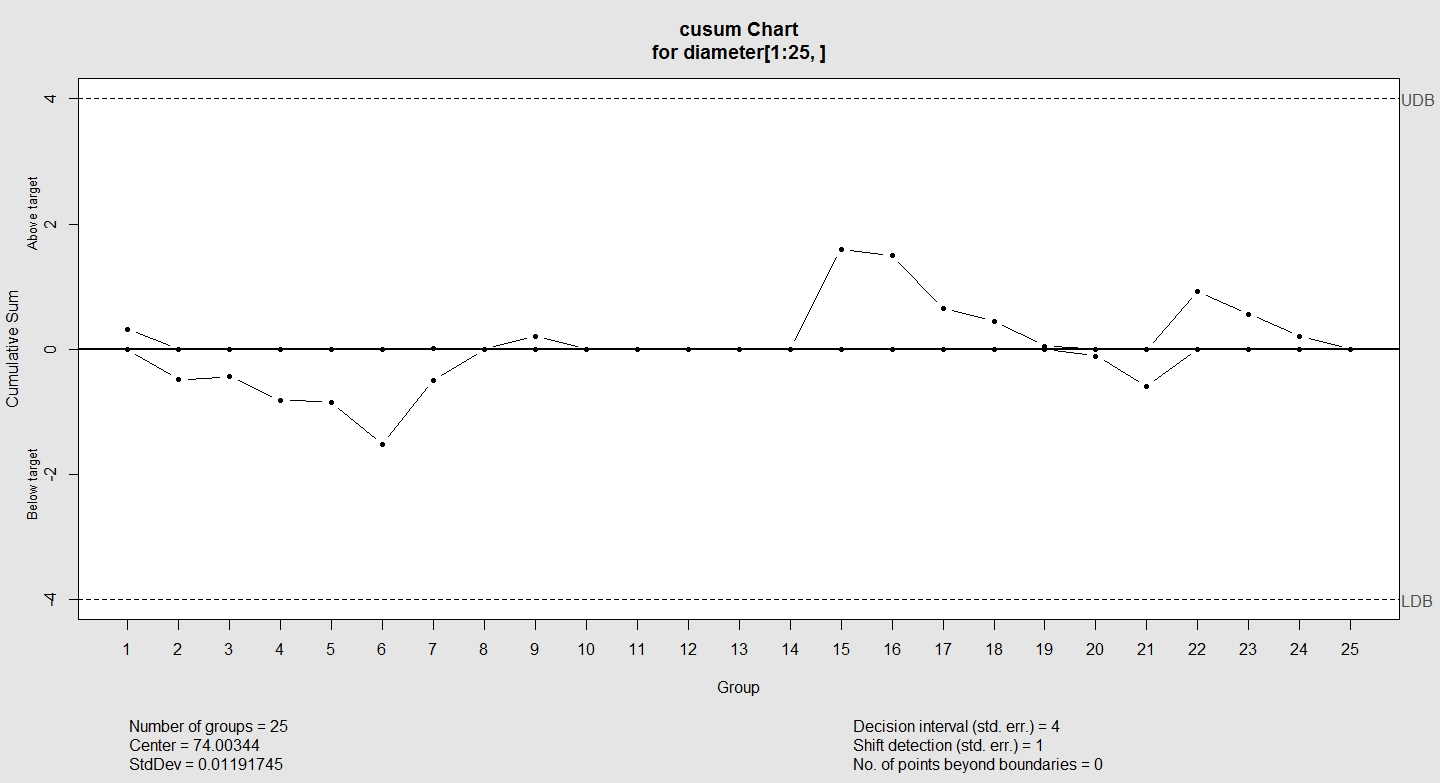
\includegraphics[width=0.9\linewidth]{images/CUSUMorings1}
\caption{}
\label{fig:cusumorings1}
\end{figure}
\begin{figure}[h!]
\centering
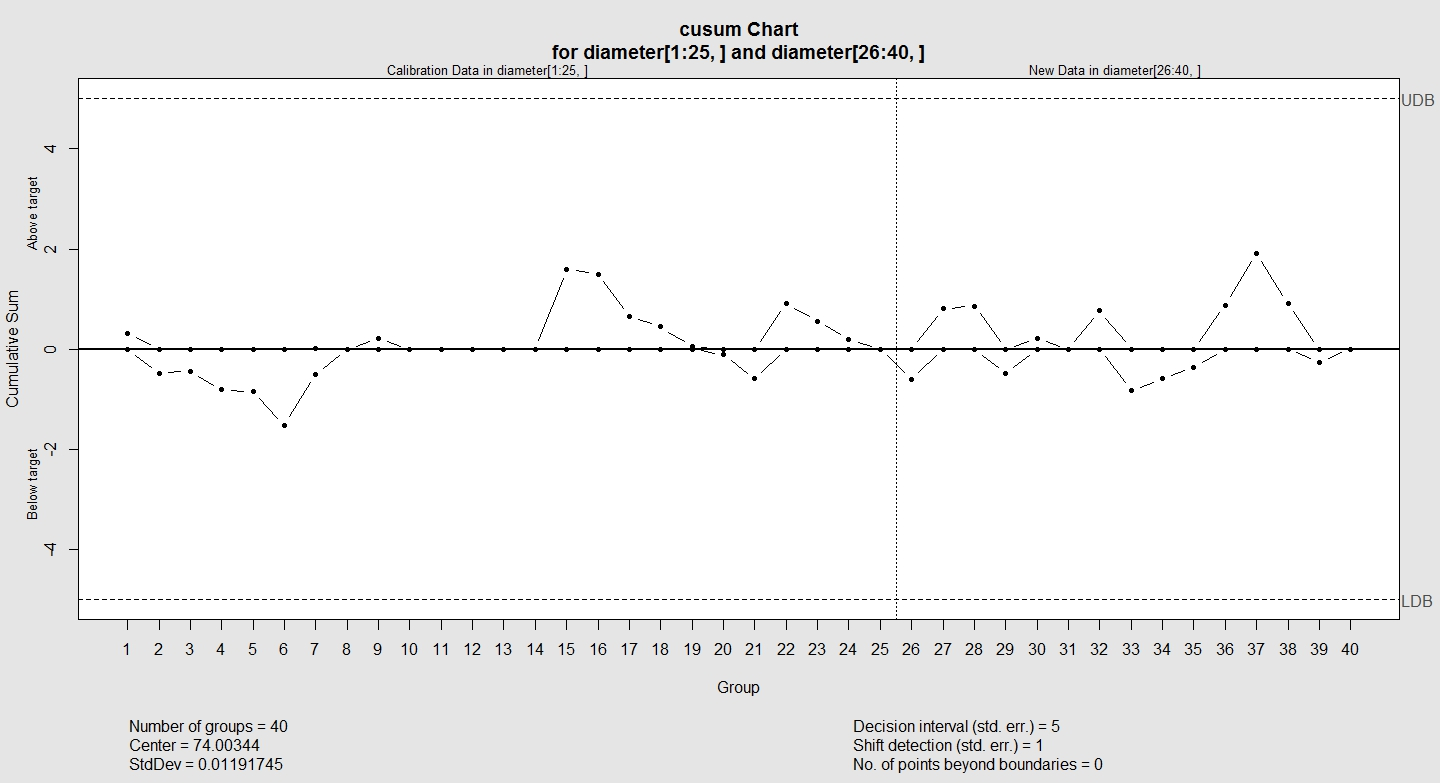
\includegraphics[width=0.9\linewidth]{images/CUSUMorings2}
\caption{}
\label{fig:cusumorings2}
\end{figure}

\newpage

\subsection{Average Run Length}
The sensitivity of \textbf{h} is calculated from the \textit{\textbf{averaged run length (arl)}}. This is the averaged number of measurements between each false alarm when the situation is still in control.
\end{document}
